\chapter{Databázový model}

\begin{figure}[H]
	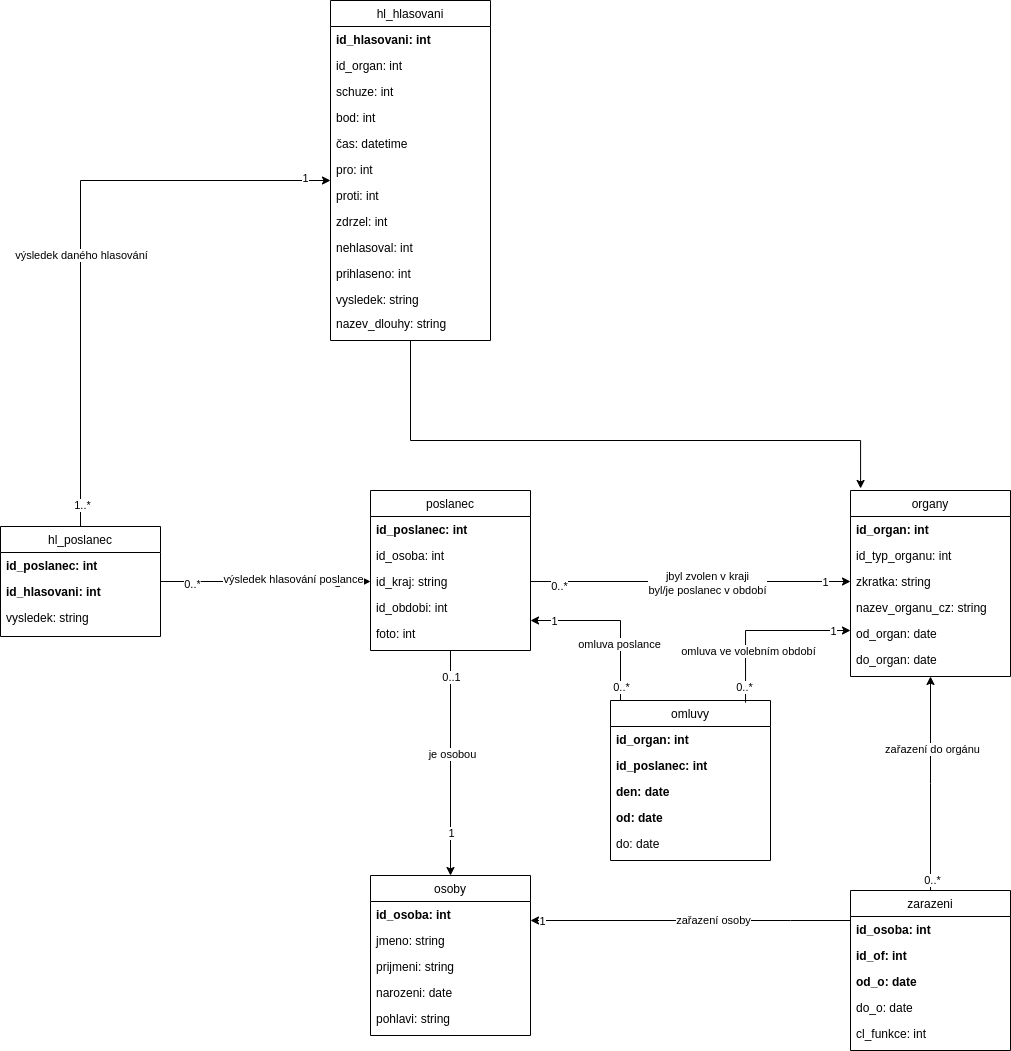
\includegraphics[width=\linewidth]{source_data_diagram}
	\caption{Diagram zdrojových dat PSP}
	\label{fig:class-diagram}
\end{figure}

\begin{table}[!h]\centering
	\caption[Struktura agency]{Struktura agency}\label{table:agency}
	\begin{tabular}{|l|l|p{6cm}|}\hline
		Název	& Typ	& Popis	\tabularnewline \hline \hline
		\texttt{id}		& \texttt{int}	& identifikátor orgánu		\tabularnewline \hline
		\texttt{abbreviation}		& \texttt{varchar(255)}	& zkratka názvu orgánu		\tabularnewline \hline
		\texttt{end\textunderscore date}		& \texttt{date(255)}	& datum zániku orgánu		\tabularnewline \hline
		\texttt{name}		& \texttt{varchar(255)}	& název orgánu		\tabularnewline \hline
		\texttt{start\textunderscore date}		& \texttt{date}	& datum založení orgánu		\tabularnewline \hline
		\texttt{type\textunderscore id}		& \texttt{int}	& identifikátor typu orgánu 		\tabularnewline \hline
	\end{tabular}
\end{table}

\begin{table}[!h]\centering
	\caption[Struktura excuse]{Struktura excuse}\label{table:excuse}
	\begin{tabular}{|l|l|p{6cm}|}\hline
		Název	& Typ	& Popis	\tabularnewline \hline \hline
		\texttt{member\textunderscore id}		& \texttt{int}	& identifikátor poslance, který je omluven		\tabularnewline \hline
		\texttt{date} & \texttt{date}	& datum, kdy je poslanec omluven \tabularnewline \hline
		\texttt{start\textunderscore time}		& \texttt{time}	& čas, od kterého byl poslanec omluven \tabularnewline \hline
		\texttt{end\textunderscore time}		& \texttt{time}	& čas, do kterého byl poslanec omluven \tabularnewline \hline
		\texttt{election\textunderscore year}		& \texttt{int}	& volební rok \tabularnewline \hline
	\end{tabular}
\end{table}

\begin{table}[!h]\centering
	\caption[Struktura member]{Struktura member}\label{table:member}
	\begin{tabular}{|l|l|p{6cm}|}\hline
		Název	& Typ	& Popis	\tabularnewline \hline \hline
		\texttt{id}		& \texttt{int}	& identifikátor poslance, který je omluven		\tabularnewline \hline
		\texttt{date\textunderscore of\textunderscore birth} & \texttt{date}	& datum narození \tabularnewline \hline
		\texttt{election\textunderscore region}		& \texttt{varchar(255)}	& volební kraj \tabularnewline \hline
		\texttt{election\textunderscore year}		& \texttt{int}	& volební rok \tabularnewline \hline
		\texttt{gender}		& \texttt{varchar(255)}	& pohlaví \tabularnewline \hline
		\texttt{member\textunderscore from} & \texttt{date} & datum začátku členství \tabularnewline \hline
		\texttt{member\textunderscore to} & \texttt{date} & datum konce členství \tabularnewline \hline
		\texttt{name} & \texttt{varchar(255)} & jméno \tabularnewline \hline
		\texttt{person\textunderscore id} & \texttt{int} & identifikátor osoby \tabularnewline \hline
		\texttt{photo\textunderscore url} & \texttt{varchar(255)} & URL profilové fotky \tabularnewline \hline
		\texttt{source\textunderscore url} & \texttt{varchar(255)} & URL oficiálního zdroje \tabularnewline \hline
		\texttt{party\textunderscore id} & \texttt{int} & identifikíátor poslaneckého klubu, jehož je členem \tabularnewline \hline
	\end{tabular}
\end{table}

\begin{table}[!h]\centering
	\caption[Struktura member\textunderscore vote]{Struktura member\textunderscore vote}\label{table:membe_vote}
	\begin{tabular}{|l|l|p{6cm}|}\hline
		Název	& Typ	& Popis	\tabularnewline \hline \hline
		\texttt{result}		& \texttt{varchar(255)}	& jak hlasoval poslanec\tabularnewline \hline
		\texttt{member\textunderscore id}		& \texttt{int}	& jak identifikátor poslance\tabularnewline \hline
		\texttt{vote\textunderscore id}		& \texttt{int}	& identifikátor hlasování\tabularnewline \hline
	\end{tabular}
\end{table}

\begin{table}[!h]\centering
	\caption[Struktura membership]{Struktura membership}\label{table:membership}
	\begin{tabular}{|l|l|p{6cm}|}\hline
		Název	& Typ	& Popis	\tabularnewline \hline \hline
		\texttt{end\textunderscore date}		& \texttt{datetime}	& datum a čas konce zařazení\tabularnewline \hline
		\texttt{agency\textunderscore id}		& \texttt{int}	& identifikátor orgánu\tabularnewline \hline
		\texttt{person\textunderscore id}		& \texttt{int}	& identifikátor osoby \tabularnewline \hline
		\texttt{start\textunderscore date}		& \texttt{datetime}	& datum a čas začátku zařazení \tabularnewline \hline
	\end{tabular}
\end{table}

\begin{table}[!h]\centering
	\caption[Struktura party]{Struktura party}\label{table:party}
	\begin{tabular}{|l|l|p{6cm}|}\hline
		Název	& Typ	& Popis	\tabularnewline \hline \hline
		\texttt{abbreviation} & \texttt{varchar(255)} & zkratka pro název klubu\tabularnewline \hline
		\texttt{name} & \texttt{varchar(255)}	& název klubu\tabularnewline \hline
		\texttt{election\textunderscore year}		& \texttt{int}	& volební rok \tabularnewline \hline
		\texttt{party\textunderscore id}		& \texttt{int}	& identifikátor klubu \tabularnewline \hline
	\end{tabular}
\end{table}

\begin{table}[!h]\centering
	\caption[Struktura vote]{Struktura vote}\label{table:vote}
	\begin{tabular}{|l|l|p{6cm}|}\hline
		Název	& Typ	& Popis	\tabularnewline \hline \hline
		\texttt{date\textunderscore time} & \texttt{datetime} & datum a čas hlasování\tabularnewline \hline
		\texttt{description} & \texttt{varchar(255)}	& popis hlasování\tabularnewline \hline
		\texttt{election\textunderscore year}		& \texttt{int}	& volební rok\tabularnewline \hline
		\texttt{excused\textunderscore count}		& \texttt{int}	& počet omluvených \tabularnewline \hline
		\texttt{logged\textunderscore off\textunderscore count}		& \texttt{int}	& počet nepřihlášených \tabularnewline \hline
		\texttt{meeting\textunderscore number}		& \texttt{int}	& bod hlasování \tabularnewline \hline
		\texttt{no\textunderscore count}		& \texttt{int}	& počet hlasování proti \tabularnewline \hline
		\texttt{refrained\textunderscore count}		& \texttt{int}	& počet zdržených \tabularnewline \hline
		\texttt{result}		& \texttt{varchar(255)}	& výsledek hlasování \tabularnewline \hline
		\texttt{steno\textunderscore protocol\textunderscore url}		& \texttt{varchar(255)}	& stenoprotokol \tabularnewline \hline
		\texttt{yes\textunderscore count}		& \texttt{int}	& počet hlasování pro \tabularnewline \hline
		\texttt{number}		& \texttt{int}	& číslo hlasování \tabularnewline \hline
		\texttt{id}		& \texttt{int}	& identifikátor hlasování \tabularnewline \hline
	\end{tabular}
\end{table}
